% !TEX program = xelatex
\documentclass[11pt]{ctexart}

\newcommand{\ReportLeftMargin}{18mm}
\newcommand{\ReportRightMargin}{18mm}
\newcommand{\ReportTopMargin}{18mm}
\newcommand{\ReportBottomMargin}{22mm}

\usepackage[
  a4paper,
  left=\ReportLeftMargin,
  right=\ReportRightMargin,
  top=\ReportTopMargin,
  bottom=\ReportBottomMargin
]{geometry}
\usepackage{fontspec}
\usepackage{graphicx}
\usepackage[table]{xcolor}
\usepackage{array}
\usepackage{tabularx}
\usepackage{booktabs}
\usepackage{tcolorbox}
\usepackage{titlesec}
\usepackage{setspace}
\usepackage{caption}
\usepackage{amssymb}
\usepackage{needspace}
\usepackage{fancyhdr}

\defaultfontfeatures{Ligatures=TeX, Scale=MatchLowercase}

\setmainfont{Baskerville}
\setsansfont{Avenir Next}
\setCJKmainfont[
  BoldFont={Hiragino Sans GB W6},
  ItalicFont={Kaiti SC}
]{STFangsong}
\setCJKsansfont[
  BoldFont={Hiragino Sans GB W6}
]{Hiragino Sans GB W3}
\newCJKfontfamily\TitleCJK[BoldFont={Lantinghei SC}]{Lantinghei SC}

\definecolor{MiraText}{HTML}{2F3640}
\definecolor{MiraMuted}{HTML}{D8DDE6}
\definecolor{MiraAccent}{HTML}{F05A4A}
\definecolor{MiraWarm}{HTML}{FFF5EB}
\definecolor{MiraWarmBorder}{HTML}{FED4A4}
\definecolor{MiraTableHead}{HTML}{F3F5F8}
\definecolor{MiraTableStripe}{HTML}{FAFBFC}

\setlength{\parindent}{0pt}
\setlength{\parskip}{0.58em}
\setstretch{1.22}
\renewcommand{\arraystretch}{1.35}

\pagestyle{fancy}
\fancyhf{}
\renewcommand{\headrulewidth}{0pt}
\cfoot{\footnotesize\sffamily\color{MiraText}\thepage}

\titleformat{\section}
  {\Large\bfseries\sffamily\TitleCJK\color{MiraText}}
  {}
  {0pt}
  {}

\titleformat{\subsection}
  {\large\bfseries\sffamily\TitleCJK\color{MiraText}}
  {}
  {0pt}
  {}

\titlespacing*{\section}{0pt}{1.3em}{0.8em}
\titlespacing*{\subsection}{0pt}{0.9em}{0.5em}

\captionsetup{font=small,labelformat=empty}
\tcbset{boxrule=0.8pt,arc=4pt,left=10pt,right=10pt,top=8pt,bottom=8pt}

\newcolumntype{Y}{>{\raggedright\arraybackslash}X}
\newcolumntype{L}[1]{>{\raggedright\arraybackslash}p{#1}}
\newlength{\FieldLabelWidth}
\setlength{\FieldLabelWidth}{6.9em}

\newcommand{\SectionDivider}{%
  \vspace{0.9em}%
  {\color{MiraMuted}\rule{\linewidth}{0.6pt}}%
  \vspace{1.05em}%
}

\newcommand{\Field}[2]{%
  \par\noindent
  \hangindent=\FieldLabelWidth
  \hangafter=1
  \makebox[\FieldLabelWidth][l]{{\sffamily\bfseries\TitleCJK #1}}#2\par
}

\newcommand{\InlineLead}[2]{%
  \textbf{#1} #2\par
}

\begin{document}
\thispagestyle{empty}

\vspace*{-\ReportTopMargin}
\noindent\makebox[\linewidth][l]{%
  \hspace*{-\ReportLeftMargin}
\includegraphics[width=\paperwidth]{assets/cover-banner.png}%
}

\vspace{1.2cm}
{\fontsize{24}{28}\selectfont\sffamily\bfseries\TitleCJK\color{MiraText} Mira 项目说明书\par}
\vspace{1.6cm}

\section*{一、项目概述}

\begin{tcolorbox}[colback=white,colframe=MiraMuted,boxrule=0.9pt,arc=5pt,left=12pt,right=12pt,top=10pt,bottom=10pt]
\Field{项目名称：}{Mira --- 世界上第一个实时感知主动照顾你的 AI 伴侣}
\Field{一句话介绍：}{Mira 通过智能穿戴设备实时感知用户状态，连接智能家居和软件主动提供个性化关怀，无需用户开口。}
\Field{Slogan：}{有些关心，不需要开口。}
\Field{赛道：}{生活龙虾 · 把日子过好}
\Field{所获荣誉：}{清华 AttraX OpenClaw 黑客松硬件赛道第一名，13 号开始开发，24h 内完成 demo 开发}
\end{tcolorbox}

\SectionDivider

\section*{二、关于 Mira 的缘起}

我是一个深度的 AI 情感陪伴产品用户。用过 Replika、Pi、Character.AI，但总觉得不够真实、不够自然。研究了很久才发现原因，AI 产品缺乏的是主动感知的能力。

主动感知的能力是什么呢 --- 小狗看到你难过就凑过来了要贴贴，闺蜜会感觉到你对旁边的男生心动，去主动帮你要微信。这些都不需要你开口。

\textbf{现有的 AI 陪伴产品缺少的，是主动感知的能力。}

\SectionDivider

\section*{三、解决什么问题}
\subsection*{谁在替他们看着？}

中国有 1.3 亿独居老人，一个人住，摔了一跤不跟孩子说。有 1700 万视障人士，出门不知道对面的人是善意还是恶意、路面的危险变化。有 900 万留守儿童，放学后没人知道他们在哪、是不是在干危险的事。有上亿独居青年，加班到深夜回到空荡荡的家，没人问一句“今天怎么样”。

这些人有一个共同点：\textbf{他们是最需要被关心的人，也是最不会主动开口的人。}

老人说“挺好的”。孩子说“没事”。年轻人说“我还行”。视障人士不想麻烦别人。

现有的 AI 陪伴产品都需要用户主动开口才能感知情绪。但这些人不会开口。

\textbf{我们需要一种新的交互方式：不等你开口，主动感知你的状态，主动照顾你。}

\SectionDivider

\section*{四、Mira 是什么}
\subsection*{世界上第一个实时感知、主动照顾的 AI 伴侣}

Mira 基于 OpenClaw 开源框架构建，通过智能穿戴设备（AR 眼镜、智能手表）实时感知用户的视觉环境和生理指标，结合对用户的长期记忆理解，由大模型自主判断用户当前状态并决定行动。同时通过 MCP 协议接入 11 大智能家居生态，将判断转化为真实世界的行动 --- 调灯光、放音乐、控温度、通知家人。

\InlineLead{核心特征：}{}
\InlineLead{实时感知：}{不是定时检查，不是阈值报警，是每秒都在看、每秒都在感受}
\InlineLead{主动照顾：}{不等用户开口，不需要用户操作任何设备}
\InlineLead{连接物理世界：}{已接入 Xiaomi、Hue、HomeKit 等 11 大智能家居生态，感知到了就能做到}
\InlineLead{个性化理解：}{同样的情况，对不同的人做不同的事 --- 基于长期记忆积累}
\InlineLead{有分寸感：}{大多数时候选择沉默，只在真正需要的时候无声出现}

\subsection*{AI 陪伴的三个阶段}

\arrayrulecolor{MiraMuted}
\rowcolors{2}{MiraTableStripe}{white}
\begin{tabularx}{\linewidth}{L{0.18\linewidth} L{0.24\linewidth} L{0.26\linewidth} Y}
\hline
\rowcolor{MiraTableHead}
\textbf{阶段} & \textbf{代表产品} & \textbf{交互方式} & \textbf{局限} \\
\hline
2024：你找它 & Replika、Character.AI & 用户主动发起对话 & 不开口就没有陪伴 \\
2025：它找你 & Pi、Friend & AI 定时推送问候 & 不知道用户实际状态 \\
2026：它懂你 & Mira & 实时感知，主动行动 & 无需交互 \\
\hline
\end{tabularx}

\SectionDivider

\section*{五、技术架构}
\subsection*{四层架构：从感知到行动}

\InlineLead{L1 感知层}{}
Rokid AR 眼镜每秒捕捉一帧画面，智能手表每秒读取一次心率，麦克风持续采集环境声音。我们改造了 OpenClaw 的 Heartbeat 系统，从每 30 分钟的响应提升到以秒为单位的实时感知。

\InlineLead{L2 记忆层}{}
感知不会立刻消散。contracts 与上下文把瞬时观察铸成结构化记忆，让“看见了什么、发生过什么、谁确认过什么”变成可追溯、可召回的时间纹理。

\InlineLead{L3 分析层}{}
在 gateway 与 plugins 之间，系统把世界翻译成判断。它区分噪声与信号、意图与风险、建议与命令。基于 Memory 积累的个性化理解，让智能不只是反应，而是理解你之后的选择。

\InlineLead{L4 执行层}{}
判断落向真实世界。Ha-Control、Hue、SmartThings 及各类执行插件通过 OpenClaw MCP 协议统一调度，已接入 11 大智能家居生态，把分析变成动作、把上下文变成编排，让一套系统真正从“看见”走向“发生”。

\SectionDivider

\section*{六、应用场景}
\subsection*{场景一：独居老人健康守护}

妈妈一个人住在老家。今天她走路比昨天慢了，在沙发上坐了三个小时没动，午饭只吃了半碗。她什么都没说。但 Mira 给远在北京工作的女儿发了一条消息：

\begin{tcolorbox}[colback=MiraTableStripe,colframe=MiraWarmBorder]
\textbf{“妈妈今天状态不太好，给她打个电话。”}
\end{tcolorbox}

女儿打了电话。妈妈说“没事没事”。但女儿听出来了 --- 因为 Mira 提醒了她去注意。

Mira 不是冷冰冰的健康监测手环。它是每天都在默默观察你妈妈的存在。

\subsection*{场景二：疲惫打工人的回家时刻}

你加班到晚上十点。Mira 通过眼镜看到你一直盯着电脑屏幕，通过手表知道你心率偏高了一整天，通过 Memory 知道你午饭没怎么吃。

当你推开家门 --- 灯光已经是暖黄色的，加湿器在吐雾，音箱在放你这周循环了二十遍的那首歌，香薰机亮着。

它什么也没有说，但最好的夜床服务已经布置好了。

\subsection*{场景三：调皮孩子的安全守护}

孩子在小区里玩，爬上了一棵树。Mira 通过摄像头检测到危险姿态，父母的手机立刻响了。

每一个需要被惦记的人，都是 Mira 的用户。

\SectionDivider

\section*{七、OpenClaw 深度集成}

Mira 是 Claw Native 的产品，深度使用了 OpenClaw 的核心能力：

\arrayrulecolor{MiraMuted}
\rowcolors{2}{MiraTableStripe}{white}
\begin{tabularx}{\linewidth}{L{0.24\linewidth} Y}
\hline
\rowcolor{MiraTableHead}
\textbf{OpenClaw 能力} & \textbf{Mira 的使用方式} \\
\hline
\textbf{Memory} & 存储用户的长期理解 --- 性格、习惯、偏好、社交关系 \\
\textbf{Heartbeat} & 从 30 分钟改造为秒级持续感知循环 \\
\textbf{MCP 协议} & 统一调度 11 大智能家居生态 \\
\textbf{Gateway} & 接收眼镜和手表的实时数据流 \\
\textbf{Skills 系统} & Mira 的感知引擎作为 OpenClaw 的新型 Skill \\
\hline
\end{tabularx}

\textbf{Mira 是 OpenClaw 生态中第一个面向情感关怀方向的应用。} OpenClaw 的 13000+ 个 Skill 全部面向效率工具，Mira 填补了“AI 关怀”这个空白品类。

\SectionDivider

\section*{八、安全与隐私}
\subsection*{安全 360°：四层防护}

更强的感知能力意味着更大的隐私责任。我们建立了四层安全防护体系：

\InlineLead{L1 云服务器安全：}{IP 白名单访问 · 双重认证 · HTTPS 全链路加密}
\InlineLead{L2 OpenClaw 加固：}{Shell 沙箱封装限制命令范围 · 权限最小化 · 安全审计插件}
\InlineLead{L3 AI 行为约束：}{rejection.md 明确禁止行为清单 · Memory 中写入安全指令 · 沉默优先原则}
\InlineLead{L4 终端设备控制：}{设备白名单授权 · 所有数据本地处理不上传云端 · 视频帧分析完即销毁 · 用户随时可暂停感知和清除记忆}

\textbf{核心原则：Mira 感知你是为了照顾你，不是为了监控你。用户是数据的唯一所有者。}

\SectionDivider

\section*{九、社会价值}
\subsection*{社会价值}

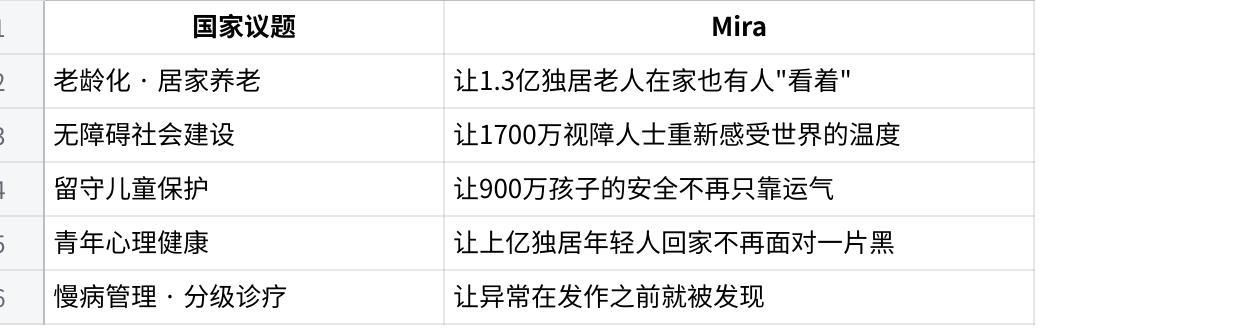
\includegraphics[width=\linewidth]{assets/social-value-table.png}

\begin{center}
\textbf{点击图片可查看完整电子表格}
\end{center}

\begin{tcolorbox}[colback=MiraWarm,colframe=MiraWarmBorder]
\textcolor{MiraAccent}{\Large$\heartsuit$}\hspace{0.4em}\textbf{科技向善不是一句口号。是妈妈一个人在家的时候，有个东西在替你惦记她。}
\end{tcolorbox}

\SectionDivider

\section*{十、团队介绍}

\arrayrulecolor{MiraMuted}
\rowcolors{2}{MiraTableStripe}{white}
\begin{tabularx}{\linewidth}{L{0.20\linewidth} Y}
\hline
\rowcolor{MiraTableHead}
\textbf{成员} & \textbf{角色} \\
\hline
Rick & 产品与设计 · 连续创业者 · Wisconsin 设计 + 经济学 \\
Junkai & 后端与安全架构 \\
\hline
\end{tabularx}

\textbf{清华 OpenClaw 黑客松硬件赛道第一名}

\SectionDivider

\section*{十一、如何使用}

\begin{tcolorbox}[colback=white,colframe=MiraMuted,boxrule=0.9pt,arc=5pt,left=12pt,right=12pt,top=10pt,bottom=10pt]
\Field{项目名称：}{Mira}
\Field{Slogan：}{有些关心，不需要开口。}
\Field{英文表达：}{The care before the ask.}
\Field{加入方式：}{Join Mira World · 欢迎扫码加入}
\end{tcolorbox}

\end{document}
